
Le but du stage était de manipuler les intégrales de choquet et les résaux de neurones.
La prédiction du prix des maisons à été étudiée grâce à une base de donnée trouvée sur internet\cite{houses}.
On pourait tout simplement multiplier le prix au metre carré par la superficie de la maison
mais on verra par la suite que cette technique est loin d'être optimale.


\section{Un petit point théorique\ldots}
\label{sec:th}
Afin de mieux comprende les interactions entre les differentes notions,
un petit point théorique est necessaire :
\begin{itemize}
    \item Compréhention du fonctionnement d'un réseau de neurones
    \item Fonctionnement des intégrales de choquet
    \item Pourquoi les integrales de choquet associées aux résaux de neurones sont particulierement efficace pour résoudre certains problèmes
\end{itemize}

\subsection{Réseaux de neurones}\label{subsec:réseau-de-neurones}

Les médias parlent souvent d'intelligence artificielle et de réseaux de neurones,
ces deux notions sont radicalement différentes
mais elles sont souvent mélangées et confondues sur la place publique\ldots \\


L'intelligence artificielle est un concept informatique, un paradigme de programmation,
cette notion n'a pas été abordée durant mon stage, il n'en sera pas question ici.
Cependant si vous voulez en savoir plus, je vous redirige vers la chaine youtube de Lê \textsc{Nguyên Hoang}.
Anciennement chercheur en mathématiques et aujourd'hui vulgarisateur sur internet et à l'\textsc{EPFL}
ses vidéos sont à regarder sans moderation\cite{science4all}. \\


Un réseau de neurones est une architecture informatique inventée en 1950 et remis à la mode grâce aux travaux
de Yan \textsc{Le Cun} durant les années 1980 permettant de faire des régressions de fonctions,
de la généralisation et de l'optimisation.
Il est composé, comme son nom l'indique, de neurones mis en réseau grâce à des connexions.\\
Il va donc être d'abord abordé la notion de neurone, puis la mise en réseau.


\subsubsection{Un neurone}
Un neurone est une unité de base du réseau, il se décompose en trois phases :
\begin{itemize}
    \item L'entrée
    \item La fonction interne
    \item La fonction d'activation
\end{itemize}
Elles s'agencent de la manière suivante :
\begin{figure}[H]
    \center
    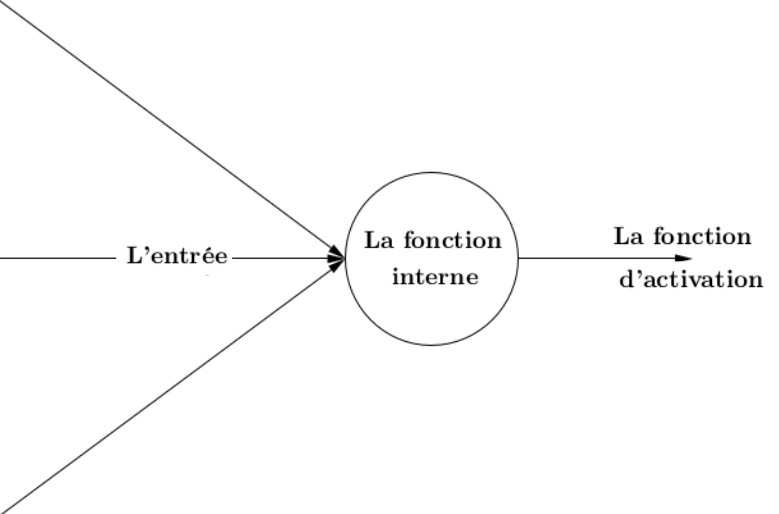
\includegraphics[height=\moyen]{pict/neurone.png}
	\caption{Un neurone}
    \label{fig:neurone}
\end{figure}


\paragraph{L'entrée :}
Un neurone prend des informations en entrée, de manière générale un nombre réel entre $0$ et $1$
mais d'autres objets sont envisageables (image, pixel, son\ldots).
Il n'y a pas de nombre minimum ou maximum
(il peut être conçu un neurone ne prenant pas d'entrée, ou au contraire en prenant une infinité),
ni de contrainte sur les différents objets.
\exemle
{
Un neurone prenant :
\begin{itemize}
    \item les valeurs de couleur d'un pixel (entier entre $0$ et $255$).
    \item les valeurs de couleur d'un pixel (réel $[0, 1]$).
    \item une sequence \textsc{adn} en entrée

\end{itemize}
}
Le vecteur entrée est noté $X$ et chacun de ses element $x_1 \ldots x_i \ldots x_n$.

\paragraph{La fonction interne :}
Le réseau va donc faire un calcul à partir des entrées.
Soit $f(X)$ la fonction interne du réseau (avec $X$ le vecteur d'entrée).
La fonction peut contenir des paramètres notés $w_1 \ldots w_i \ldots w_n$ et contenus dans le vecteur $W$.
Ces valeurs définies pour chaque neurones peuvent varier durant l'apprentissage.

\exemle
{
\begin{itemize}
    \item[$f(X) =$] $W\cdot X = \sum_{i=1}^{n} w_i \times x_i $
    \item[$f(X) =$] $\max(X)$
    \item[$f(X) =$] "nombre d'adénine sur les $w_1$ premières bases de $x_1$" \\
            (avec $x_1$ une sequence \textsc{adn})
\end{itemize}
}


\paragraph{La fonction d'activation :}
Rappelons que ces neurones sont mis en réseau.
Il est donc intéressant d'avoir une norme pour l'entrée et la sortie
afin de pouvoir lier des neurones entre eux sans distinctions.
La norme qui a été choisie est, comme précédement introduit, un réel entre $0$ et $1$.


Or, il peut être remarqué que les fonctions ci-dessus ne renvoient pas
forcement des nombres strictements compris entre $0$ et $1$.
La fonction d'activation est donc utilisée pour normaliser les sorties.
\exemle
{
\begin{itemize}
    \item[Pour une fonction dans $\mathbb{R}$ :] fonction sigmoide
    \item[Pour une fonction dans $[0, 1 \rbrack$ :] fonction identité
    \item[Pour le cas précédent sur l'\textsc{adn} :] $f(X)/w_1$
\end{itemize}
}
La fonction d'activation est noté $f_{act}$.


\paragraph{Pour resumer :}
Un neurone prend des valeurs en \textit{entrée},
les transforme via sa \textit{fonction principale},
puis retourne le résultat grâce à la \textit{fonction d'activation}. \\
Formellement, l'équation suivante est obtenue :
\begin{equation}
    f_{act}(f(X))
\end{equation}


Le tout dépendant bien évidemment du vecteur $W$ qui varie afin de modifier la fonction du neurone.
\exemle
{
Prenons un neurone avec deux entrées : $x_1$ et $x_2$, \\
de fonction principale $f(X) = X.W$ \\
et de fonction d'activation identité. \\
Si $W = (1, 1)$, ce neurone fait une somme.\\
Mais si $W = (0.5, 0.5)$ ce neurone fait une moyenne.
}


\subsubsection{Un réseau}
Une fois que nous avons de nombreux neurones faisant chacun des actions bien spécifiques,
il pourrait être intéressant de les relier afin de gérer des comportements plus complexes
comme faire une somme de moyenne (ou controller un drone, prédire les mouvements boursiers\ldots).

Il suffit donc de relier les neurones entre eux, de manière générale de manière linéaire de gauche à droite.
De nombreuse manière de relier les neurones existent (récurent, convolution\ldots),
ici il sera abordé en détail que de la connexion dite \emph{Dense} ou \emph{fully connected} :
le réseau se découpe en $n$ couches de neurones,
chacunes composée de neurones dont les entrées sont les sorties des neurones le la couche précédente.
\begin{figure}[H]
    \center
    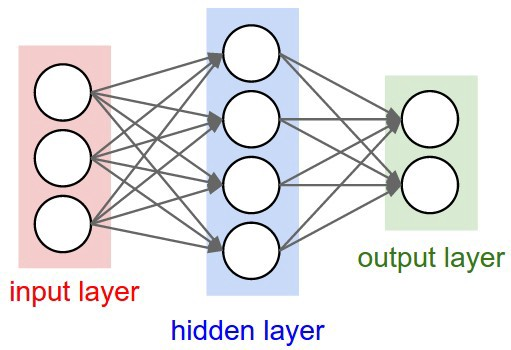
\includegraphics[height=\moyen]{pict/net1.jpeg}
	\caption{Réseau dense simple}
    {\footnotesize \url{techburst.io/experiment-finding-objects-with-a-neural-network-caa4cec7d2c4}}
	\label{fig:simple-dense}
\end{figure}
La \textsc{Figue}\ \ref{fig:simple-dense} représente un réseau fully connected :
les neurones les plus à gauches sont les neurones d'entrée (capteurs)
et ceux les plus à droite ceux de sortie (controle des moteurs, affichage d'une note\ldots).
Tous les autres neurones sont "cachés", ils n'intéragissent pas directement avec l'environnement.


\subsubsection{L'apprentissage}
Jusqu'ici il a été abordé la création d'une architecture modulable permettant de générer une fonction à paramètres.
Mais une question se pose toujours :\\
Quel est l'intérêt ?
Pourquoi ne pas directement écrire la fonction "en dur" ?\\
La réponse tient en quatre mots : \textit{Descente de gradient stochastique} (ou  \sgd\ en anglais). \\
Ce concept est ce qui fait que les réseaux de neurones sont les architectures favorites
des data scientists et des chercheurs en \textsc{ia}.\\


L'idée est assez simple, une fonction générale est cherché à partir de certaines valeurs discretes.
Posons une fonction nommé "loss function" qui décrit la précision du réseau actuel :
elle prend en entrée deux valeurs : la valeur théorique et la valeur obtenue.
Elle retourne un réel positif, plus il est faible, plus le réseau est proche de la fonction théorique.
\exemle
{
Avec $exp$ le résultat attendu et $obt$ le résultat obtenu :
\begin{align*}
    loss(exp, obt) = &\ |exp - obt| \\
    loss(exp, obt) = &\ (exp - obt)^2
\end{align*}
}
Le problème de régression se résume donc à minimiser la fonction de perte,
c'est ici que la descente de gradient stochastique fait son entrée :


\paragraph{Descente de gradient :}
Pour minimiser loss, il serait bien de descendre sa pente, c'est-à-dire dériver suivant les différentes variables
\footnote{\textsc{NB :} Ici les variables suivant lesquelles la dérivée se fait sont les $w_i$ (pas les $x_i$).},
en déduire l'orientation de la pente et la descendre.
Étant donnés que de manière générale, il y a plusieurs variables, la dérivée se transforme en gradient.
Des applications linéaires sont privilégiées dans les fonctions des neurones,
afin de pouvoir calculer facilement les gradients.\\


\paragraph{Stochastique :}
Il a été expliqué d'où vient la descente de gradient, mais que veut dire stochastique ?
Ce mot est synonyme de hasard.
En effet le temps de calcul du gradient est exponentiel vu que chaque neurones est relié a $n$ neurones,
eux même reliés à $n$ autres neurones\ldots\\
Donc lorsque le réseau est grand
(un réseau peut facilement atteindre le million de neurones voir même des milliards\cite{i3espectrum})
il est inimaginable de calculer la totalité du gradient (les calculs peuvent parfois depasser
plusieurs fois la durée de l'univers\ldots),
le gradient stochastique est donc utilisé pour rendre le calcul réalisable.\\


Cette descente de gradient est bien plus rapide, il est donc possible de l'itérer de nombreuses fois
pour tenter de minimiser la fonction de perte.
L'espace des solutions étant rarement idéal
(rarement une "cuvette" mais constitué de "bosses" et de "trous" chaotiques)
il n'est pas obligatoire d'arriver à atteindre le minimum global, mais au moins minimum local sera atteint.
Avec plusieurs apprentissages il peut donc être approximé très efficacement quasiment toutes les fonctions.


\newpage


\subsection{Intégrales de choquet}\label{subsec:intégrales-de-choquet}

L'integrale de choquet est une intégrale découlant de la théorie de la mesure\cite{artch}.
Ici on ne parlera que du modele discret.\\


Pour l'expliquer simplement, prenons un exemple :
Suposons que l'on veuille conseiller des personnes sur l'achat d'ordinateurs.
Ces personnes de conaissent absolument rien en informatique.
La seul chose qu'ils veullent est une note, plus elle est élevée, plus l'ordinateur est performant.
Essayons de faire un algorithme assez simple pour résoudre ce problemme :
Chaque composant se voit atribué une note (en fonction de la puissance, la qualité de fabrication\ldots),
on appelle cette note \textit{l'utilité} du composant.
Une fois toutes les utilitées étudiées, on donne un poid à chaque famille de composants
(\textsc{ram}, processeur, carte mère\ldots).
Enfin on fait la somme de utilité fois poid pour tout les composant.\\
De ce fait, si un ordinateur a de meilleurs composant, plus de puissance, ect, sa note sera superieure.\\


Ce modèle parait raisonable dans la plupart des cas mais il est extraimement mauvais dans les cas extremes :
Suposons qu'un constructeur peu scrupuleux propose un ordinateur assez étrange :
Le processeur le moins cher du marché (assez mauvais) mais énormément de \textsc{ram}, par exemple $128$Go.
Votre classement le placera forcément en haut de la liste, même si vous en conviendrez,
cet ordinateur est assez inutile\ldots\\


Il faudrait donc trouver un autre système modélisant les interactions entre les composants.
Ce modèle est exactement celui sur lequel j'ai travaillé durant mon stage: \textit{les intégrales de choquet}.
En plus de donner un poid aux utilité,
un poid est donné aux interactions des utilitées par le biais des fonctions min et max.
Ces intéractions peuvent être faites deux à deux, trois à trois voir à plus.
Mais pour des raison de temps de calcul, ces interactions se sont limités à l'interactions simple
(deux à deux) durant mon stage.
En effet, la taille du calcul évolue exponentiellement avec les interactions.\\


Voici donc la fonction que l'on vas vouloir aproximer :
\begin{equation}
    \label{eq:choquet}
    C(X)  =
    \sum_{i=1}^{n}
        w_i \times x_i +
    \sum_{i=1}^{n}\sum_{j=i+1}^{n}
    \Big(
        w_{M\,ij} \times \max(x_i,x_j) + w_{m\,ij} \times \min(x_i,x_j)
    \Big)
\end{equation}
Avec $X$ le vecteur des utilitées et $W$, $W_m$ et $W_M$ les vecteurs des poids.

